Objekto padėties nustatymas turi dvi plačias pritaikymo sritis: inercinė navigacinė ir žmogaus judesio sekimo sistema \cite{schlomer2008gesture};

Objekto pozicijos nustatymas, panaudojus inercinius jutiklius remiasi prielaida, jog objektas lieka ramybės būsenoje tol, kol jį nepaveikia išorinė jėga. Tokia jėga suteikia objektui pagreitį. Jeigu rasta pagreitį galima išmatuoti ir suintegruoti, pagreičio ir pozicijos kitimas gali būti išmatuoti. Reikia nepamiršti, kad tokiu atveju matavimą sudarys dvi komponentės -- pagreitis dėl gravitacijos ir išorinės veikiančios jėgos pagreitis. Norint pašalinti gravitacijos komponentę iš pagreičio matavimo, reikia žinoti kokiu kampu akcelerometras yra vertikalės atžvilgiu.
Tokio kampo matavimui, reikalingas kitas jutiklis, kuris vadinasi giroskopas. Jis matuoja kampo greitį, kurį matematiškai integruojant, galima rasti kampo greičio pokytį nuo pradinio, žinomo kampo \cite{sukkarieh2000low}.

Akcelerometras suteikia pagreičio matavimą norimam objektui. Dažniausiai tokie matavimai yra užrašomi $x$, judėjimą tiesiai, $y$, šonu ir $z$ vertikaliai. Giroskopas suteikia matavimus, kurie dengia nurodytas ašis ir yra užrašomi $\theta$, sūkiui, $\beta$ polinkiui ir $\gamma$ vingiavimui, kaip pavaizduota \ref{tikz:axis_of_the_system} pavyzdyje. Tokių inercinių įverčių naudojimas turi pagrindinį privalumą -- stebimo objekto polinkis ir pagreitis gali būti vertinami bet kokioje navigacijoje.  

\begin{figure}[H]
    \centering
    \caption{Objekto pozicijos pagreičio pokyčio ašys, $x$, $y$ ir $z$. Sūkio matmenys apie ašis $\theta$, $\beta$ ir $\gamma$.}
    \label{tikz:axis_of_the_system}
    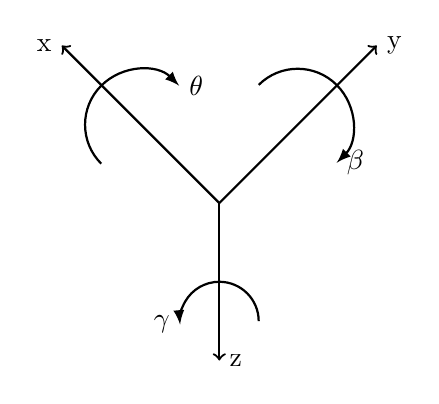
\begin{tikzpicture}
        % axis
        \draw[thick, black, ->] (0,0) -- ( 2, 2) node [right] {y};
        \draw[thick, black, ->] (0,0) -- (-2, 2) node [left] {x}; 
        \draw[thick, black, ->] (0,0) -- ( 0,-2) node [right] {z};
        % arc
        \draw[thick, -latex] ( 0.5,  1.5) arc (135:-45:0.70) node [right] {$\beta$}; 
        \draw[thick, -latex] (-1.5,  0.5) arc (225:45:0.70) node [right] {$\theta$};
        \draw[thick, -latex] ( 0.5, -1.5) arc (0:185:0.5) node [left] {$\gamma$};
    \end{tikzpicture}
\end{figure}

Inercinės navigacijos sistemos yra naudojamos labai plačiai lėktuvuose, raketose, kosmoso laivuose, povandeniniuose ir vandens laivuose \cite{woodman2007introduction}. Progresas gaminant MEMS įrenginius, sudarė galimybes kurti mažas ir lengvas navigacines sistemas. Tokie privalumai leidžia praplatinti įrenginių panaudojimo galimybes ir šiuo metu įtraukia tokias sritis kaip žmogaus ir gyvūnų judesio sekimą.

Tačiau reikia nepamiršti ir apie klaidas, kurias sukelia nuolatinė dedamoji, santykio įverčiai ir nelinijines sistemos įtakos jutiklio verčių nuskaitymo metu. Tokios klaidos yra pagrindinė priežastis atsirasti netikslumams navigacinėje sistemoje per laiko vienetą. Netikslumai sąlygoja akselerometro įverčius, kuriuos tampa labai sunku atskirti tarp gravitacinio lauko ir objekto judėjimo, ko pasekoje objekto pozicijos matavimas toliau yra dar netikslesnis. Kadangi inerciniai jutikliai yra tokio tipo, kuriems yra labai svarbi tiksli prieš tai buvusi pozicija, bet kokia klaida skaičiuojant prieš tai buvusia pozicija, įtakoja ir dabartinės pozicijos skaičiavimą. Tokiu būdu, su laiku navigacinė sistema tampa visiškai netiksli ir praranda visą savo vertę.